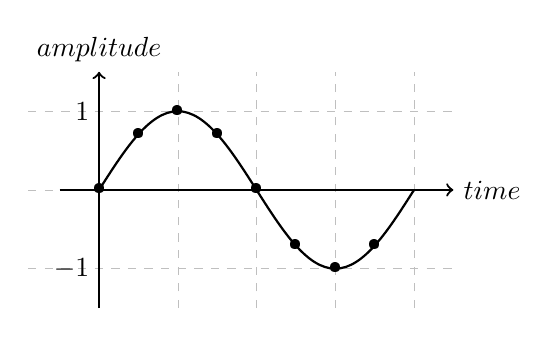
\begin{tikzpicture}
\draw[help lines, color=gray!50, dashed ] (-0.9,-1.5) grid (4.5,1.5);
\draw[->,thick] (-0.5,0)--(4.5,0) node[right]{$time$};
\draw[->,thick] (0,-1.5)--(0,1.5) node[above]{$amplitude$};
\draw(0,1) node[left] {$1$};
\draw(0,-1) node[left] {$-1$};
\draw[thick] (0,0) sin (1,1);
\draw[thick] (1,1) cos (2,0);
\draw[thick] (2,0) sin (3,-1);
\draw[thick] (3,-1) cos (4,0);
\foreach \Point in {(0,0),(0.5,0.707),(1,1),(1.5,0.707),(2,0),(2.5,-0.707),(3,-1),(3.5,-0.707)}{
    \node at \Point {\textbullet};
}
\end{tikzpicture}